\section{NVIDIA GPU 硬件与软件层级结构及 CUDA 介绍}

本章将深入探讨 NVIDIA GPU 的硬件与软件层级结构，并介绍 CUDA。

CUDA 全称为 Compute Unified Device Architecture（统一计算设备架构），是由 NVIDIA 开发的一个并行计算平台和应用程序编程
接口（API）。CUDA 允许软件开发者使用 NVIDIA 的图形处理单元进行通用目的计算，这种方法被称为 GPGPU（General-Purpose 
computing on Graphics Processing Units，即图形处理单元上的通用计算）。

在开始之前，强调三个关键点。第一，CUDA 基于 C 编程语言，这是一个优势，它让熟悉 C 语言的开发者能够轻松编写可在 
NVIDIA GPU 上执行的软件。第二是 CUDA 编译器 \texttt{nvcc}——它不仅仅是一个普通的编译器，而是 CUDA 工具包的核心。
\texttt{nvcc} 的作用远不止将 CUDA 代码转换为可执行文件或机器码，它在开发过程中扮演着多重关键角色。随着本课程的推进，
我们将逐步揭示 \texttt{nvcc} 的多功能性，以及它如何优化 CUDA 应用程序。

第三点是主机（Host）与设备（Device）这两个术语的区别，这是为了充分利用 GPU 的资源。通常，主机指的是 CPU 及其关联的
全局内存（即 RAM），而设备则指 GPU 及其全局内存。这种区分不仅在术语上非常重要，在编写软件的方式上也至关重要——它影响
代码结构、数据传输和内存管理。本图中左侧部分代表主机，右侧部分代表设备（即 GPU）。

\begin{figure}
    \centering
    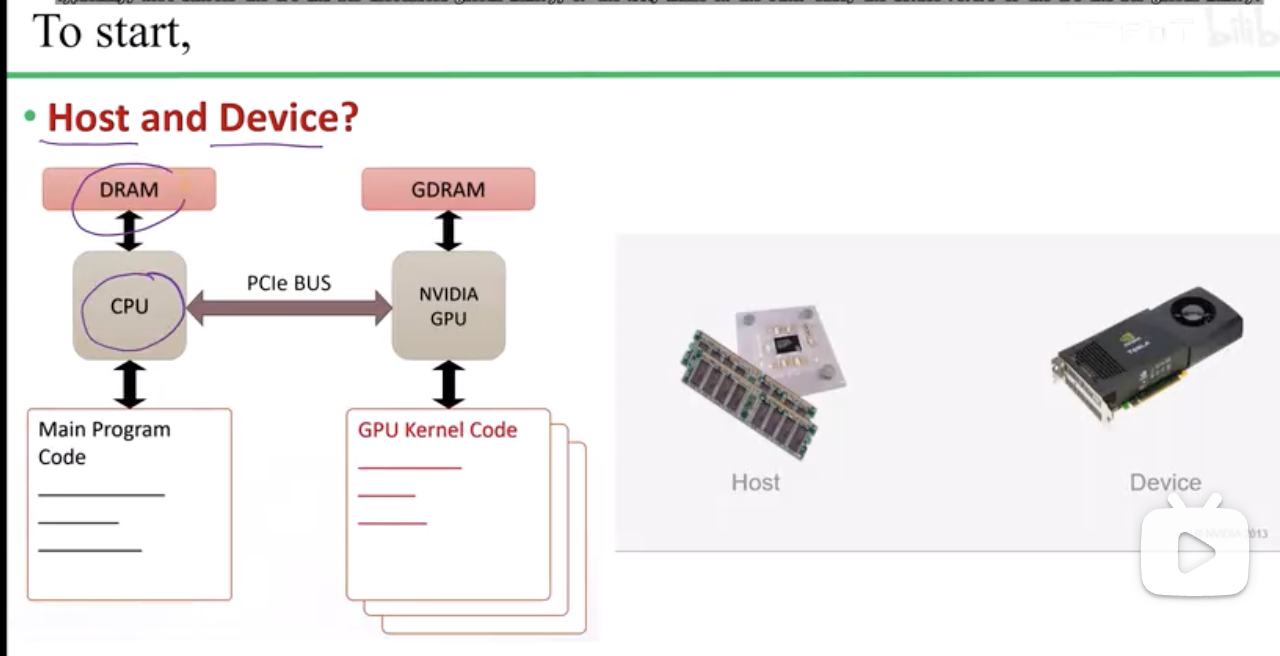
\includegraphics[width=0.75\linewidth]{resources/cuda-061.png}
    \caption{}
    \label{fig:placeholder}
\end{figure}

\subsection{硬件四级层级}

回顾 GPU 硬件架构层级与其软件部分之间的关系。GPU 的结构包含四个明确的硬件组织层级，且是分层的：最顶层是 GPU 本身
，它封装了所有单元；每个 SM（Streaming Multiprocessor，流式多处理器）构成该层级结构的第二级。这一设计已在 Volta 
白皮书章节中详细说明。

接着，每个 SM 又被进一步划分为若干个分区（Sub-partition / Processing Block），构成硬件结构的第三级。在 Volta 和 
Ampere 架构中，每个 SM 包含四个这样的分区。如图所示，来自 Volta 白皮书的图中 SM 被划分为四个分区。Ampere 白皮书
中也能看到类似的结构。

\begin{figure}
    \centering
    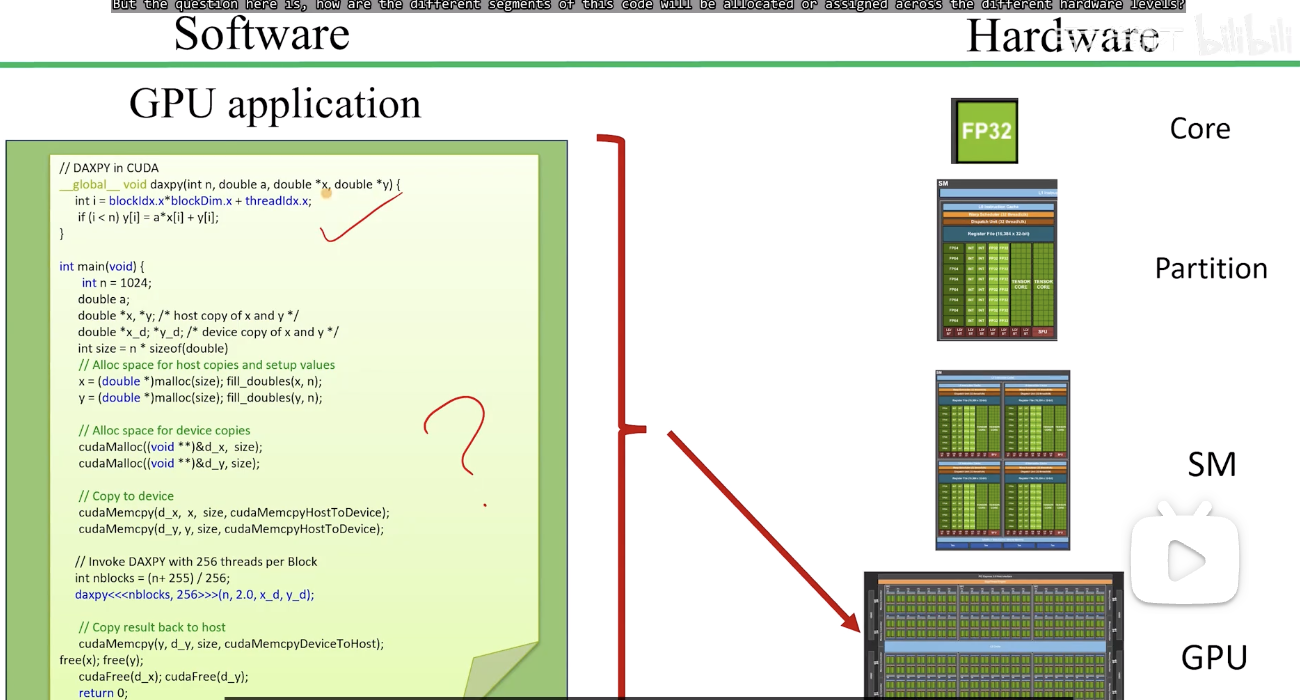
\includegraphics[width=0.75\linewidth]{resources/cuda-062.png}
    \caption{}
    \label{fig:placeholder}
\end{figure}


在第四级（最细粒度的层级），每个分区内包含独立的计算单元，例如负责执行浮点运算的 FP32 核心。这些核心是 GPU 内部处理
计算的基本单元。

综上所述，GPU 的硬件架构可视为一个四级层级结构：从整个 GPU 开始逐级向下，经过 SM，再到其内部的分区作为第三级，最终到
达各个独立的计算核心。这些不同的硬件层级反过来要求对应的软件应用程序具备相似的结构。

例如，假设我们有一个 CUDA 应用程序（如图所示，用方框表示），该应用程序设计用于在整个 GPU 上运行。问题是：这段代码的
不同部分将如何分配或指派到不同的硬件层级？这正是需要理解的内容——软件代码的不同部分如何映射到硬件的不同层级。

\begin{figure}
    \centering
    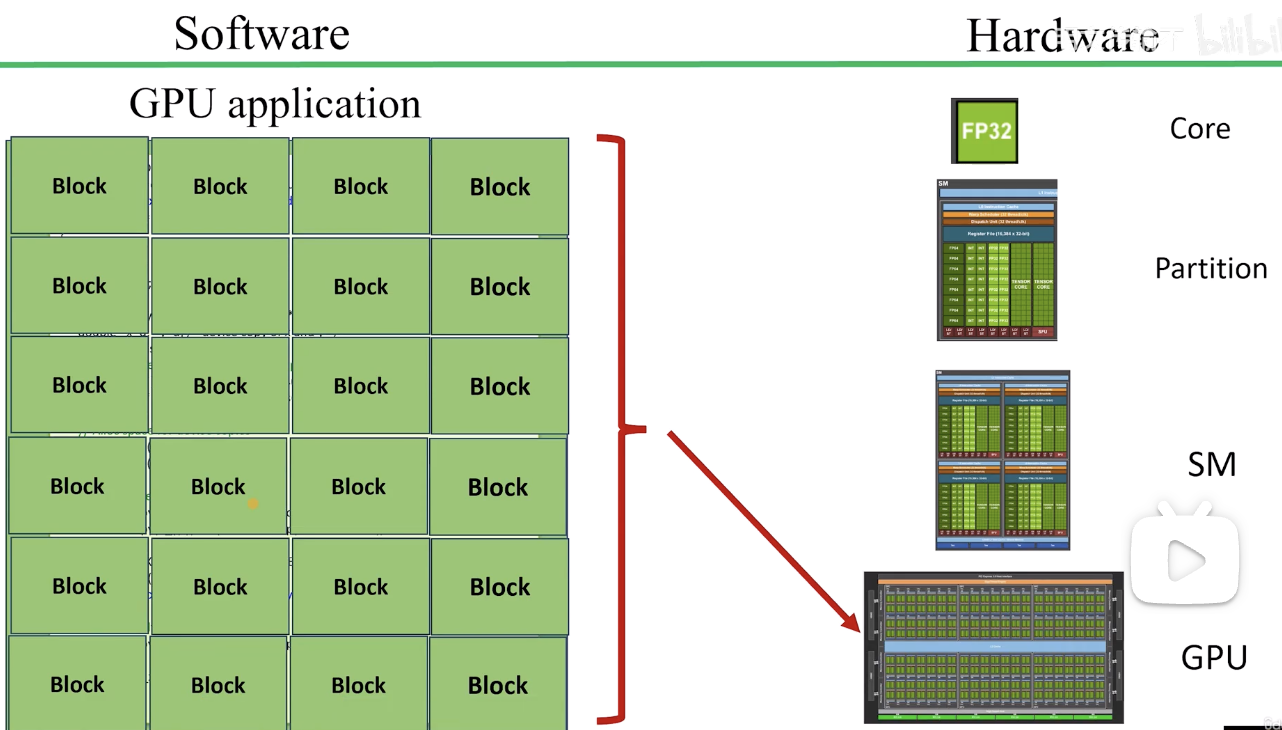
\includegraphics[width=0.75\linewidth]{resources/cuda-063.png}
    \caption{}
    \label{fig:placeholder}
\end{figure}


\subsection{软件层级：块与GigaThread Engine}

编写 CUDA 代码的第一步是将 GPU 核函数（Kernel）划分成更小的软件单元，称为块（Block）或线程块（Thread Block）。对于每
个核函数，首先需要配置其块数量。如果将整个方框视为一个 CUDA 应用程序，就可以将其划分为更小的块。如图所示，每个小方框
代表一个块（或线程块，两个名称均正确）。这种划分对应了 GPU 的前两个硬件层级——整个应用程序设计用于在整个 GPU 上执行。

然而这引发了一个问题：软件中的第二级是指不同的块在不同的 SM 上执行。在左侧，有由软件块（线程块）表示的任务；在另一侧
，有可视为"工人"的 SM。谁负责将这些软件任务分配给工人（SM）？

\begin{figure}
    \centering
    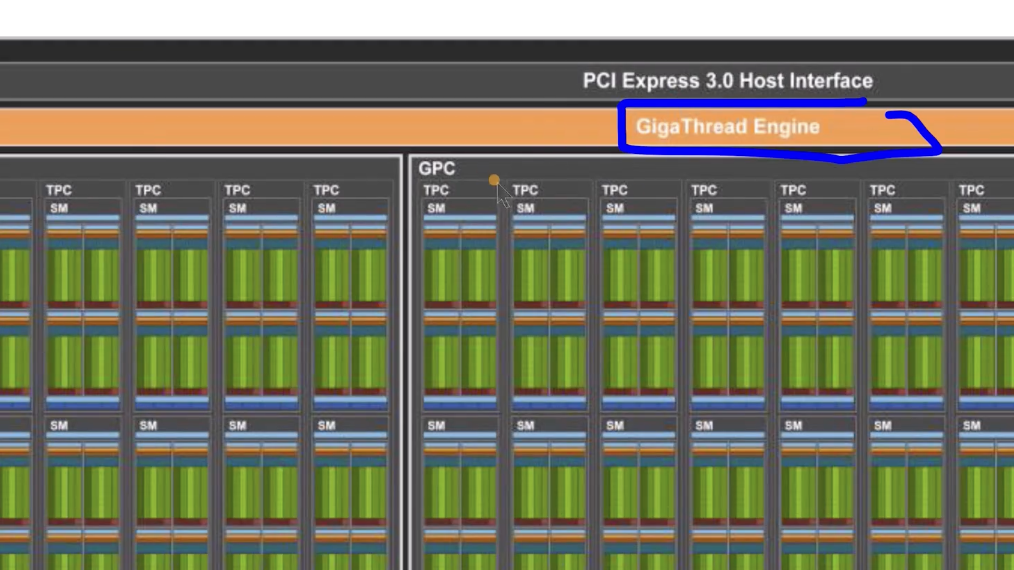
\includegraphics[width=0.75\linewidth]{resources/cuda-064.png}
    \caption{}
    \label{fig:placeholder}
\end{figure}


要回答这个问题，需要了解另一个单元——GigaThread Engine。它是 GPU 内部最重要的单元之一，其关键功能就是高效地将这些软
件块（任务/作业）分配到各个 SM 上。参考 Volta 白皮书可以看到，GigaThread Engine 位于整个 GPU 的整体结构之中，并连接到
所有 SM——它负责为这些 SM 提供必要的软件块或软件任务。

将同样的原理应用到下一层级。假设图中的第一个块被分配到某个 SM 上执行，但该 SM 中有四个分区，而我们这里只有一个块。这
个被称为"块"的单一软件单元应如何分配到 SM 内部的四个硬件分区中？

如果将整个块只分配给其中一个分区，就会导致资源利用率不足（三个分区空闲）。这一考虑引出了软件层级的第三级——Warp（线程束），以避免浪费可用的硬件资源。

\begin{figure}
    \centering
    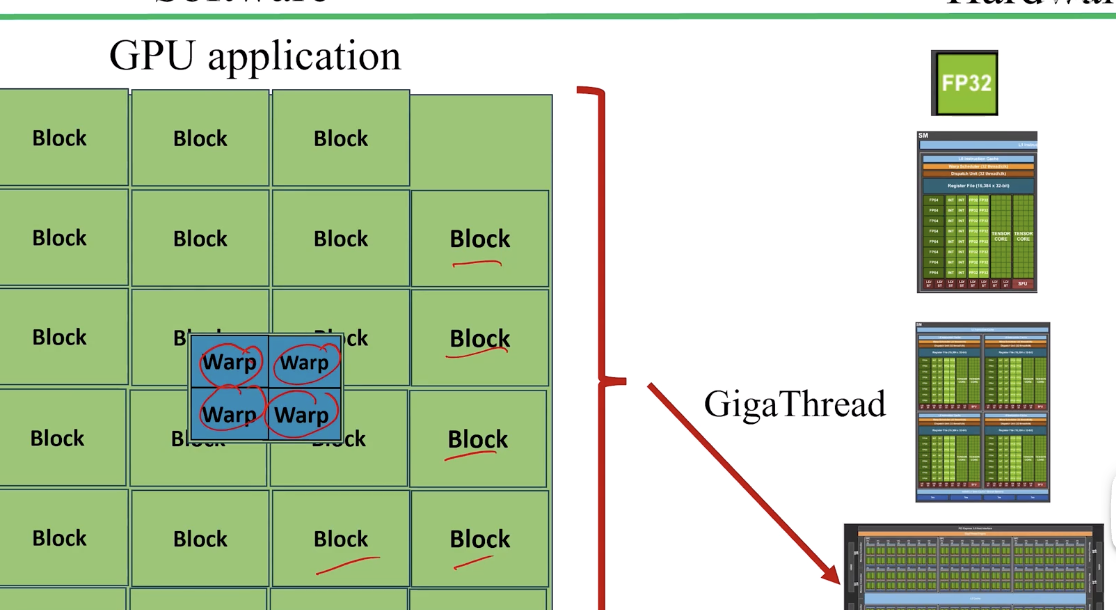
\includegraphics[width=0.75\linewidth]{resources/cuda-065.png}
    \caption{}
    \label{fig:placeholder}
\end{figure}

\subsection{Warp与调度}

每个软件块都会被细分为更小的单元，称为 Warp。例如，如果将第一个块划分为四个 Warp，那么每个 Warp 就可以分配到 SM 中的
一个不同分区——四个 Warp 对应四个分区，每个分区分配一个 Warp。

考虑另一个例子：如果每个块有 32 个 Warp，而有四个分区，那么每个分区将执行八个 Warp。当一个分区分配了多个 Warp 时，就
需要一个管理者——这就是为什么每个分区中都有一个 Warp Scheduler（Warp 调度器）单元。

放大该分区，可以看到内部的 Warp 调度器单元。正如前文所述，该单元存在于每个分区中，负责在每个时钟周期中调度某个 Warp
。这是在硬件层面；而在软件层面，一个 Warp 默认通常由 32 个线程组成。

进入第四级，每个分区包含若干个核心。Warp 中的每个线程会在分区内独立的核心上执行，确保每个核心都积极参与计算。理解硬件
和软件中的这四个层级，对于高效配置 CUDA 应用程序至关重要。

块的数量以及每个块中的线程数量，是启动任何 CUDA 应用程序时需要指定的两个关键参数（将在后续章节中详细探讨）。关于 Warp
，可以通过将块大小（即每个块的线程数）除以 32 来计算每个块中的 Warp 数量，因为 Warp 的大小固定为 32 个线程。
